\documentclass[1p]{elsarticle_modified}
%\bibliographystyle{elsarticle-num}

%\usepackage[colorlinks]{hyperref}
%\usepackage{abbrmath_seonhwa} %\Abb, \Ascr, \Acal ,\Abf, \Afrak
\usepackage{amsfonts}
\usepackage{amssymb}
\usepackage{amsmath}
\usepackage{amsthm}
\usepackage{scalefnt}
\usepackage{amsbsy}
\usepackage{kotex}
\usepackage{caption}
\usepackage{subfig}
\usepackage{color}
\usepackage{graphicx}
\usepackage{xcolor} %% white, black, red, green, blue, cyan, magenta, yellow
\usepackage{float}
\usepackage{setspace}
\usepackage{hyperref}

\usepackage{tikz}
\usetikzlibrary{arrows}

\usepackage{multirow}
\usepackage{array} % fixed length table
\usepackage{hhline}

%%%%%%%%%%%%%%%%%%%%%
\makeatletter
\renewcommand*\env@matrix[1][\arraystretch]{%
	\edef\arraystretch{#1}%
	\hskip -\arraycolsep
	\let\@ifnextchar\new@ifnextchar
	\array{*\c@MaxMatrixCols c}}
\makeatother %https://tex.stackexchange.com/questions/14071/how-can-i-increase-the-line-spacing-in-a-matrix
%%%%%%%%%%%%%%%

\usepackage[normalem]{ulem}

\newcommand{\msout}[1]{\ifmmode\text{\sout{\ensuremath{#1}}}\else\sout{#1}\fi}
%SOURCE: \msout is \stkout macro in https://tex.stackexchange.com/questions/20609/strikeout-in-math-mode

\newcommand{\cancel}[1]{
	\ifmmode
	{\color{red}\msout{#1}}
	\else
	{\color{red}\sout{#1}}
	\fi
}

\newcommand{\add}[1]{
	{\color{blue}\uwave{#1}}
}

\newcommand{\replace}[2]{
	\ifmmode
	{\color{red}\msout{#1}}{\color{blue}\uwave{#2}}
	\else
	{\color{red}\sout{#1}}{\color{blue}\uwave{#2}}
	\fi
}

\newcommand{\Sol}{\mathcal{S}} %segment
\newcommand{\D}{D} %diagram
\newcommand{\A}{\mathcal{A}} %arc


%%%%%%%%%%%%%%%%%%%%%%%%%%%%%5 test

\def\sl{\operatorname{\textup{SL}}(2,\Cbb)}
\def\psl{\operatorname{\textup{PSL}}(2,\Cbb)}
\def\quan{\mkern 1mu \triangleright \mkern 1mu}

\theoremstyle{definition}
\newtheorem{thm}{Theorem}[section]
\newtheorem{prop}[thm]{Proposition}
\newtheorem{lem}[thm]{Lemma}
\newtheorem{ques}[thm]{Question}
\newtheorem{cor}[thm]{Corollary}
\newtheorem{defn}[thm]{Definition}
\newtheorem{exam}[thm]{Example}
\newtheorem{rmk}[thm]{Remark}
\newtheorem{alg}[thm]{Algorithm}

\newcommand{\I}{\sqrt{-1}}
\begin{document}

%\begin{frontmatter}
%
%\title{Boundary parabolic representations of knots up to 8 crossings}
%
%%% Group authors per affiliation:
%\author{Yunhi Cho} 
%\address{Department of Mathematics, University of Seoul, Seoul, Korea}
%\ead{yhcho@uos.ac.kr}
%
%
%\author{Seonhwa Kim} %\fnref{s_kim}}
%\address{Center for Geometry and Physics, Institute for Basic Science, Pohang, 37673, Korea}
%\ead{ryeona17@ibs.re.kr}
%
%\author{Hyuk Kim}
%\address{Department of Mathematical Sciences, Seoul National University, Seoul 08826, Korea}
%\ead{hyukkim@snu.ac.kr}
%
%\author{Seokbeom Yoon}
%\address{Department of Mathematical Sciences, Seoul National University, Seoul, 08826,  Korea}
%\ead{sbyoon15@snu.ac.kr}
%
%\begin{abstract}
%We find all boundary parabolic representation of knots up to 8 crossings.
%
%\end{abstract}
%\begin{keyword}
%    \MSC[2010] 57M25 
%\end{keyword}
%
%\end{frontmatter}

%\linenumbers
%\tableofcontents
%
\newcommand\colored[1]{\textcolor{white}{\rule[-0.35ex]{0.8em}{1.4ex}}\kern-0.8em\color{red} #1}%
%\newcommand\colored[1]{\textcolor{white}{ #1}\kern-2.17ex	\textcolor{white}{ #1}\kern-1.81ex	\textcolor{white}{ #1}\kern-2.15ex\color{red}#1	}

{\Large $\underline{12a_{0296}~(K12a_{0296})}$}

\setlength{\tabcolsep}{10pt}
\renewcommand{\arraystretch}{1.6}
\vspace{1cm}\begin{tabular}{m{100pt}>{\centering\arraybackslash}m{274pt}}
\multirow{5}{120pt}{
	\centering
	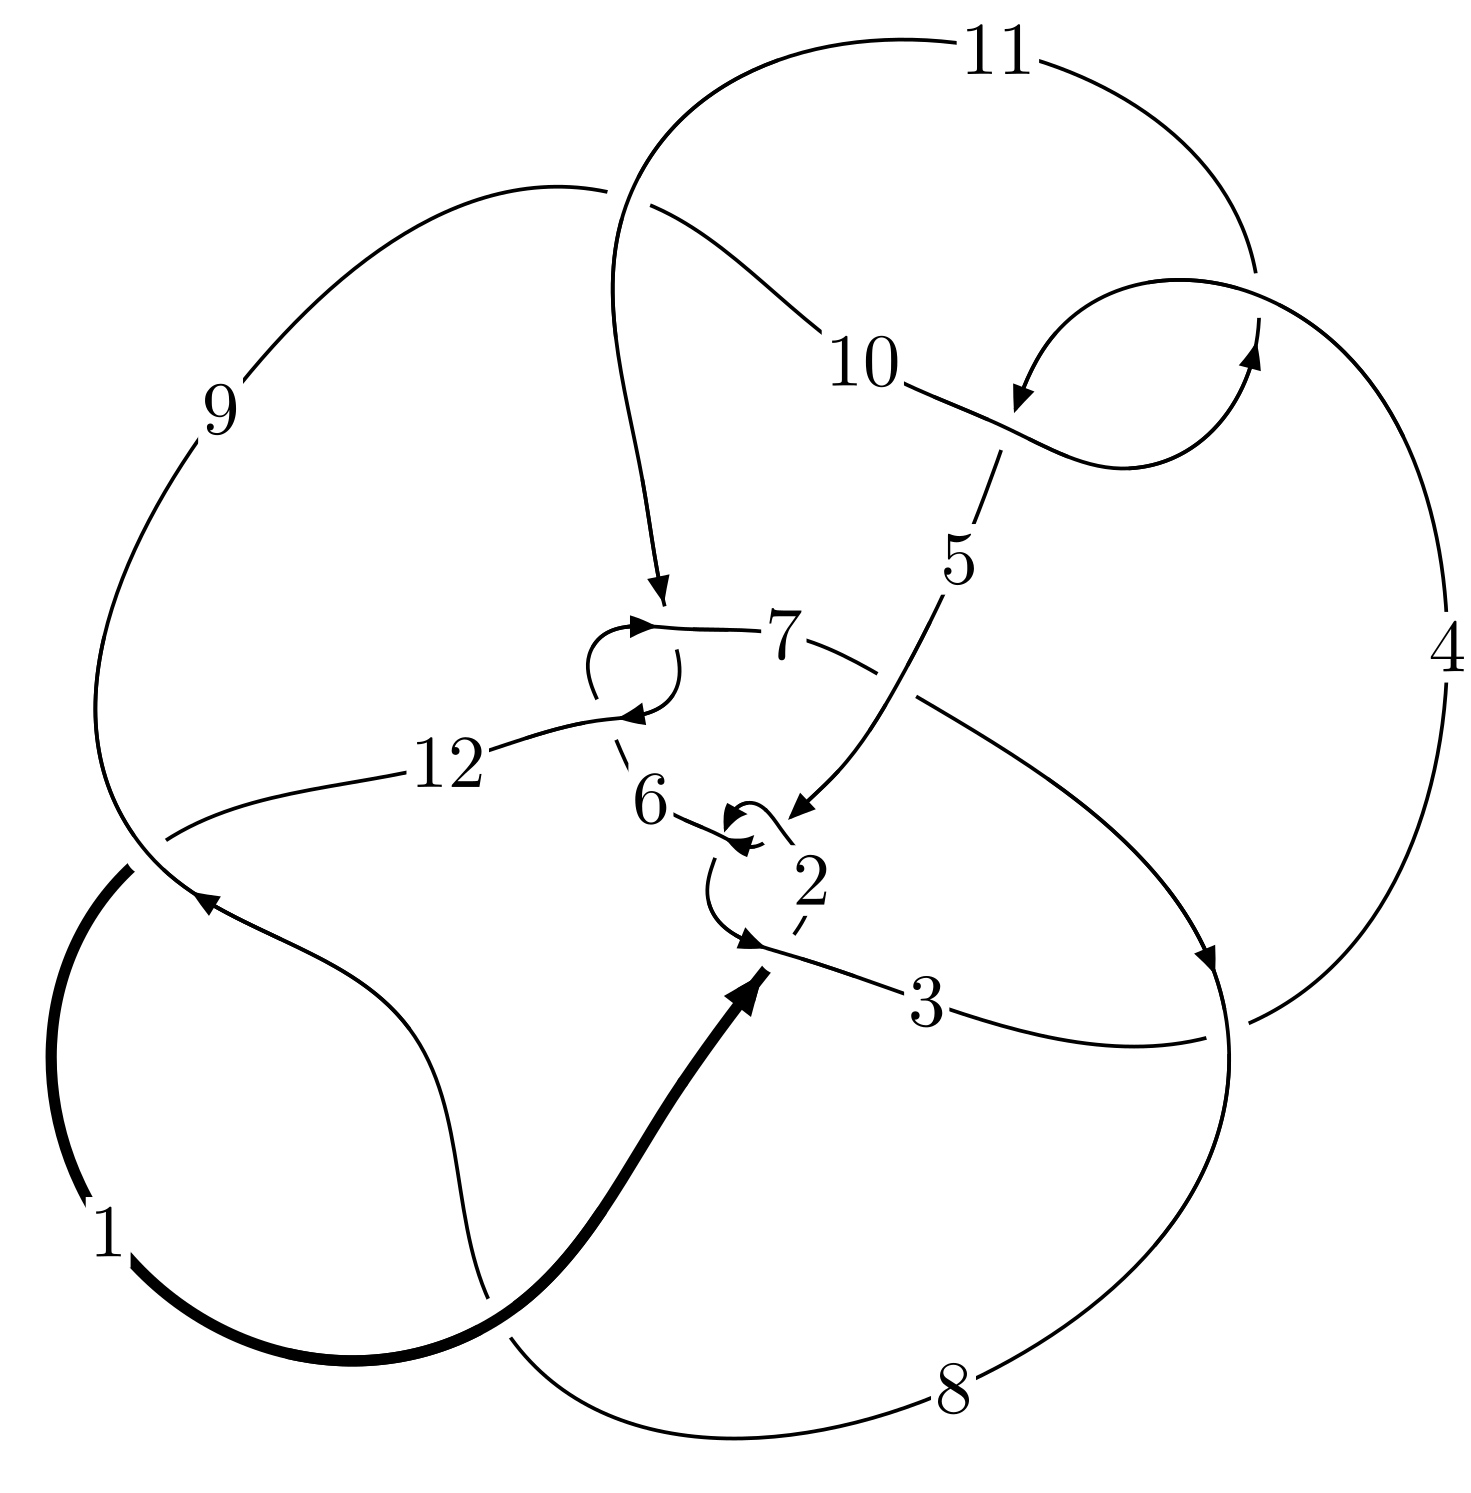
\includegraphics[width=112pt]{../../../GIT/diagram.site/Diagrams/png/1097_12a_0296.png}\\
\ \ \ A knot diagram\footnotemark}&
\allowdisplaybreaks
\textbf{Linearized knot diagam} \\
\cline{2-2}
 &
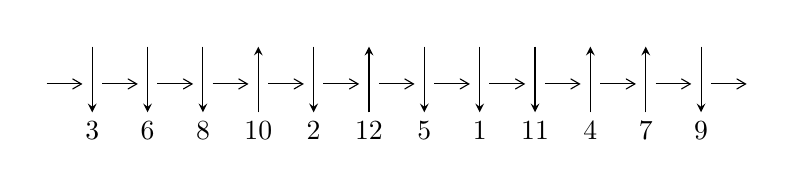
\begin{tikzpicture}[x=20pt, y=17pt]
	% nodes
	\node (C0) at (0, 0) {};
	\node (C1) at (1, 0) {};
	\node (C1U) at (1, +1) {};
	\node (C1D) at (1, -1) {3};

	\node (C2) at (2, 0) {};
	\node (C2U) at (2, +1) {};
	\node (C2D) at (2, -1) {6};

	\node (C3) at (3, 0) {};
	\node (C3U) at (3, +1) {};
	\node (C3D) at (3, -1) {8};

	\node (C4) at (4, 0) {};
	\node (C4U) at (4, +1) {};
	\node (C4D) at (4, -1) {10};

	\node (C5) at (5, 0) {};
	\node (C5U) at (5, +1) {};
	\node (C5D) at (5, -1) {2};

	\node (C6) at (6, 0) {};
	\node (C6U) at (6, +1) {};
	\node (C6D) at (6, -1) {12};

	\node (C7) at (7, 0) {};
	\node (C7U) at (7, +1) {};
	\node (C7D) at (7, -1) {5};

	\node (C8) at (8, 0) {};
	\node (C8U) at (8, +1) {};
	\node (C8D) at (8, -1) {1};

	\node (C9) at (9, 0) {};
	\node (C9U) at (9, +1) {};
	\node (C9D) at (9, -1) {11};

	\node (C10) at (10, 0) {};
	\node (C10U) at (10, +1) {};
	\node (C10D) at (10, -1) {4};

	\node (C11) at (11, 0) {};
	\node (C11U) at (11, +1) {};
	\node (C11D) at (11, -1) {7};

	\node (C12) at (12, 0) {};
	\node (C12U) at (12, +1) {};
	\node (C12D) at (12, -1) {9};
	\node (C13) at (13, 0) {};

	% arrows
	\draw[->,>={angle 60}]
	(C0) edge (C1) (C1) edge (C2) (C2) edge (C3) (C3) edge (C4) (C4) edge (C5) (C5) edge (C6) (C6) edge (C7) (C7) edge (C8) (C8) edge (C9) (C9) edge (C10) (C10) edge (C11) (C11) edge (C12) (C12) edge (C13) ;	\draw[->,>=stealth]
	(C1U) edge (C1D) (C2U) edge (C2D) (C3U) edge (C3D) (C4D) edge (C4U) (C5U) edge (C5D) (C6D) edge (C6U) (C7U) edge (C7D) (C8U) edge (C8D) (C9U) edge (C9D) (C10D) edge (C10U) (C11D) edge (C11U) (C12U) edge (C12D) ;
	\end{tikzpicture} \\
\hhline{~~} \\& 
\textbf{Solving Sequence} \\ \cline{2-2} 
 &
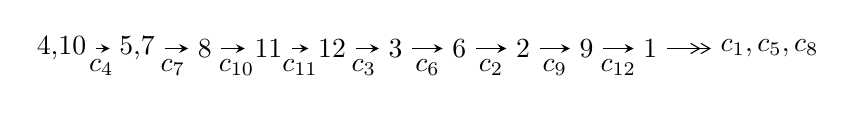
\begin{tikzpicture}[x=23pt, y=7pt]
	% node
	\node (A0) at (-1/8, 0) {4,10};
	\node (A1) at (17/16, 0) {5,7};
	\node (A2) at (17/8, 0) {8};
	\node (A3) at (25/8, 0) {11};
	\node (A4) at (33/8, 0) {12};
	\node (A5) at (41/8, 0) {3};
	\node (A6) at (49/8, 0) {6};
	\node (A7) at (57/8, 0) {2};
	\node (A8) at (65/8, 0) {9};
	\node (A9) at (73/8, 0) {1};
	\node (C1) at (1/2, -1) {$c_{4}$};
	\node (C2) at (13/8, -1) {$c_{7}$};
	\node (C3) at (21/8, -1) {$c_{10}$};
	\node (C4) at (29/8, -1) {$c_{11}$};
	\node (C5) at (37/8, -1) {$c_{3}$};
	\node (C6) at (45/8, -1) {$c_{6}$};
	\node (C7) at (53/8, -1) {$c_{2}$};
	\node (C8) at (61/8, -1) {$c_{9}$};
	\node (C9) at (69/8, -1) {$c_{12}$};
	\node (A10) at (11, 0) {$c_{1},c_{5},c_{8}$};

	% edge
	\draw[->,>=stealth]	
	(A0) edge (A1) (A1) edge (A2) (A2) edge (A3) (A3) edge (A4) (A4) edge (A5) (A5) edge (A6) (A6) edge (A7) (A7) edge (A8) (A8) edge (A9) ;
	\draw[->>,>={angle 60}]	
	(A9) edge (A10);
\end{tikzpicture} \\ 

\end{tabular} \\

\footnotetext{
The image of knot diagram is generated by the software ``\textbf{Draw programme}" developed by Andrew Bartholomew(\url{http://www.layer8.co.uk/maths/draw/index.htm\#Running-draw}), where we modified some parts for our purpose(\url{https://github.com/CATsTAILs/LinksPainter}).
}\phantom \\ \newline 
\centering \textbf{Ideals for irreducible components\footnotemark of $X_{\text{par}}$} 
 
\begin{align*}
I^u_{1}&=\langle 
5.66805\times10^{409} u^{150}+7.51787\times10^{409} u^{149}+\cdots+5.35159\times10^{409} b+1.77240\times10^{412},\\
\phantom{I^u_{1}}&\phantom{= \langle  }3.44011\times10^{410} u^{150}+6.49333\times10^{411} u^{149}+\cdots+8.37524\times10^{411} a+1.88098\times10^{414},\\
\phantom{I^u_{1}}&\phantom{= \langle  }u^{151}+u^{150}+\cdots+342 u+313\rangle \\
I^u_{2}&=\langle 
-258384 u^{35}-345517 u^{34}+\cdots+229205 b+43500,\\
\phantom{I^u_{2}}&\phantom{= \langle  }-1983831 u^{35}-980862 u^{34}+\cdots+229205 a+169836,\;u^{36}+11 u^{34}+\cdots-2 u+1\rangle \\
\\
\end{align*}
\raggedright * 2 irreducible components of $\dim_{\mathbb{C}}=0$, with total 187 representations.\\
\footnotetext{All coefficients of polynomials are rational numbers. But the coefficients are sometimes approximated in decimal forms when there is not enough margin.}
\newpage
\renewcommand{\arraystretch}{1}
\centering \section*{I. $I^u_{1}= \langle 5.67\times10^{409} u^{150}+7.52\times10^{409} u^{149}+\cdots+5.35\times10^{409} b+1.77\times10^{412},\;3.44\times10^{410} u^{150}+6.49\times10^{411} u^{149}+\cdots+8.38\times10^{411} a+1.88\times10^{414},\;u^{151}+u^{150}+\cdots+342 u+313 \rangle$}
\flushleft \textbf{(i) Arc colorings}\\
\begin{tabular}{m{7pt} m{180pt} m{7pt} m{180pt} }
\flushright $a_{4}=$&$\begin{pmatrix}1\\0\end{pmatrix}$ \\
\flushright $a_{10}=$&$\begin{pmatrix}0\\u\end{pmatrix}$ \\
\flushright $a_{5}=$&$\begin{pmatrix}1\\- u^2\end{pmatrix}$ \\
\flushright $a_{7}=$&$\begin{pmatrix}-0.0410748 u^{150}-0.775301 u^{149}+\cdots-172.627 u-224.588\\-1.05913 u^{150}-1.40479 u^{149}+\cdots-523.215 u-331.192\end{pmatrix}$ \\
\flushright $a_{8}=$&$\begin{pmatrix}0.682596 u^{150}+0.0126601 u^{149}+\cdots+86.6262 u-123.209\\-0.600054 u^{150}-1.12759 u^{149}+\cdots-274.719 u-311.069\end{pmatrix}$ \\
\flushright $a_{11}=$&$\begin{pmatrix}u\\u\end{pmatrix}$ \\
\flushright $a_{12}=$&$\begin{pmatrix}1.15095 u^{150}+2.01915 u^{149}+\cdots+397.900 u+529.928\\1.33205 u^{150}+0.776008 u^{149}+\cdots+461.621 u+106.637\end{pmatrix}$ \\
\flushright $a_{3}=$&$\begin{pmatrix}-1.25934 u^{150}-2.29137 u^{149}+\cdots-702.103 u-832.025\\-1.59595 u^{150}-0.488422 u^{149}+\cdots-622.825 u-281.236\end{pmatrix}$ \\
\flushright $a_{6}=$&$\begin{pmatrix}-3.08072 u^{150}-0.428415 u^{149}+\cdots-1135.73 u+47.9606\\0.461189 u^{150}+2.50390 u^{149}+\cdots+125.479 u+745.681\end{pmatrix}$ \\
\flushright $a_{2}=$&$\begin{pmatrix}-0.685011 u^{150}-2.74856 u^{149}+\cdots-331.641 u-1006.45\\-2.28481 u^{150}-1.01482 u^{149}+\cdots-661.078 u-346.871\end{pmatrix}$ \\
\flushright $a_{9}=$&$\begin{pmatrix}u^3\\u^3+u\end{pmatrix}$ \\
\flushright $a_{1}=$&$\begin{pmatrix}1.36356 u^{150}+2.27678 u^{149}+\cdots+499.452 u+599.666\\1.46366 u^{150}+0.729837 u^{149}+\cdots+487.027 u+58.9669\end{pmatrix}$\\&\end{tabular}
\flushleft \textbf{(ii) Obstruction class $= -1$}\\~\\
\flushleft \textbf{(iii) Cusp Shapes $= -2.91848 u^{150}+2.19523 u^{149}+\cdots-604.970 u+711.664$}\\~\\
\newpage\renewcommand{\arraystretch}{1}
\flushleft \textbf{(iv) u-Polynomials at the component}\newline \\
\begin{tabular}{m{50pt}|m{274pt}}
Crossings & \hspace{64pt}u-Polynomials at each crossing \\
\hline $$\begin{aligned}c_{1}\end{aligned}$$&$\begin{aligned}
&u^{151}+67 u^{150}+\cdots+52840 u+1156
\end{aligned}$\\
\hline $$\begin{aligned}c_{2},c_{5}\end{aligned}$$&$\begin{aligned}
&u^{151}+3 u^{150}+\cdots+70 u+34
\end{aligned}$\\
\hline $$\begin{aligned}c_{3}\end{aligned}$$&$\begin{aligned}
&u^{151}+u^{150}+\cdots-179023038 u+197503417
\end{aligned}$\\
\hline $$\begin{aligned}c_{4},c_{10}\end{aligned}$$&$\begin{aligned}
&u^{151}+u^{150}+\cdots+342 u+313
\end{aligned}$\\
\hline $$\begin{aligned}c_{6},c_{11}\end{aligned}$$&$\begin{aligned}
&u^{151}-2 u^{150}+\cdots+21021 u+2741
\end{aligned}$\\
\hline $$\begin{aligned}c_{7}\end{aligned}$$&$\begin{aligned}
&u^{151}-3 u^{150}+\cdots-33752 u+4808
\end{aligned}$\\
\hline $$\begin{aligned}c_{8},c_{12}\end{aligned}$$&$\begin{aligned}
&u^{151}-4 u^{150}+\cdots+20182265 u-3589991
\end{aligned}$\\
\hline $$\begin{aligned}c_{9}\end{aligned}$$&$\begin{aligned}
&u^{151}+69 u^{150}+\cdots-1865578 u-97969
\end{aligned}$\\
\hline
\end{tabular}\\~\\
\newpage\renewcommand{\arraystretch}{1}
\flushleft \textbf{(v) Riley Polynomials at the component}\newline \\
\begin{tabular}{m{50pt}|m{274pt}}
Crossings & \hspace{64pt}Riley Polynomials at each crossing \\
\hline $$\begin{aligned}c_{1}\end{aligned}$$&$\begin{aligned}
&y^{151}+53 y^{150}+\cdots+332733400 y-1336336
\end{aligned}$\\
\hline $$\begin{aligned}c_{2},c_{5}\end{aligned}$$&$\begin{aligned}
&y^{151}-67 y^{150}+\cdots+52840 y-1156
\end{aligned}$\\
\hline $$\begin{aligned}c_{3}\end{aligned}$$&$\begin{aligned}
&y^{151}+49 y^{150}+\cdots-1753792917130715680 y-39007599726675889
\end{aligned}$\\
\hline $$\begin{aligned}c_{4},c_{10}\end{aligned}$$&$\begin{aligned}
&y^{151}+69 y^{150}+\cdots-1865578 y-97969
\end{aligned}$\\
\hline $$\begin{aligned}c_{6},c_{11}\end{aligned}$$&$\begin{aligned}
&y^{151}+88 y^{150}+\cdots-10437379 y-7513081
\end{aligned}$\\
\hline $$\begin{aligned}c_{7}\end{aligned}$$&$\begin{aligned}
&y^{151}+5 y^{150}+\cdots-2044025440 y-23116864
\end{aligned}$\\
\hline $$\begin{aligned}c_{8},c_{12}\end{aligned}$$&$\begin{aligned}
&y^{151}+112 y^{150}+\cdots+15695522090649 y-12888035380081
\end{aligned}$\\
\hline $$\begin{aligned}c_{9}\end{aligned}$$&$\begin{aligned}
&y^{151}+45 y^{150}+\cdots+55326840498 y-9597924961
\end{aligned}$\\
\hline
\end{tabular}\\~\\
\newpage\flushleft \textbf{(vi) Complex Volumes and Cusp Shapes}
$$\begin{array}{c|c|c}  
\text{Solutions to }I^u_{1}& \I (\text{vol} + \sqrt{-1}CS) & \text{Cusp shape}\\
 \hline 
\begin{aligned}
u &= \phantom{-}0.474471 + 0.873042 I \\
a &= \phantom{-}0.512707 + 0.384642 I \\
b &= -0.771309 - 0.474519 I\end{aligned}
 & -0.82739 + 1.93508 I & \phantom{-0.000000 } 0 \\ \hline\begin{aligned}
u &= \phantom{-}0.474471 - 0.873042 I \\
a &= \phantom{-}0.512707 - 0.384642 I \\
b &= -0.771309 + 0.474519 I\end{aligned}
 & -0.82739 - 1.93508 I & \phantom{-0.000000 } 0 \\ \hline\begin{aligned}
u &= -0.793266 + 0.594543 I \\
a &= \phantom{-}0.251952 - 0.851259 I \\
b &= \phantom{-}1.40537 - 0.59930 I\end{aligned}
 & \phantom{-}7.82453 + 1.40406 I & \phantom{-0.000000 } 0 \\ \hline\begin{aligned}
u &= -0.793266 - 0.594543 I \\
a &= \phantom{-}0.251952 + 0.851259 I \\
b &= \phantom{-}1.40537 + 0.59930 I\end{aligned}
 & \phantom{-}7.82453 - 1.40406 I & \phantom{-0.000000 } 0 \\ \hline\begin{aligned}
u &= -0.451572 + 0.903425 I \\
a &= -0.621995 - 0.489425 I \\
b &= \phantom{-}1.06047 - 1.11575 I\end{aligned}
 & -4.24254 - 5.82195 I & \phantom{-0.000000 } 0 \\ \hline\begin{aligned}
u &= -0.451572 - 0.903425 I \\
a &= -0.621995 + 0.489425 I \\
b &= \phantom{-}1.06047 + 1.11575 I\end{aligned}
 & -4.24254 + 5.82195 I & \phantom{-0.000000 } 0 \\ \hline\begin{aligned}
u &= \phantom{-}0.927233 + 0.342795 I \\
a &= -0.334731 - 1.190830 I \\
b &= -0.553144 - 0.137294 I\end{aligned}
 & \phantom{-}6.16809 - 2.14866 I & \phantom{-0.000000 } 0 \\ \hline\begin{aligned}
u &= \phantom{-}0.927233 - 0.342795 I \\
a &= -0.334731 + 1.190830 I \\
b &= -0.553144 + 0.137294 I\end{aligned}
 & \phantom{-}6.16809 + 2.14866 I & \phantom{-0.000000 } 0 \\ \hline\begin{aligned}
u &= \phantom{-}0.737063 + 0.707878 I \\
a &= -0.610291 - 0.635214 I \\
b &= -1.312400 - 0.070924 I\end{aligned}
 & \phantom{-}1.72737 + 0.02413 I & \phantom{-0.000000 } 0 \\ \hline\begin{aligned}
u &= \phantom{-}0.737063 - 0.707878 I \\
a &= -0.610291 + 0.635214 I \\
b &= -1.312400 + 0.070924 I\end{aligned}
 & \phantom{-}1.72737 - 0.02413 I & \phantom{-0.000000 } 0\\
 \hline 
 \end{array}$$\newpage$$\begin{array}{c|c|c}  
\text{Solutions to }I^u_{1}& \I (\text{vol} + \sqrt{-1}CS) & \text{Cusp shape}\\
 \hline 
\begin{aligned}
u &= -0.316666 + 0.978460 I \\
a &= -0.191521 + 0.203636 I \\
b &= -1.116310 + 0.715770 I\end{aligned}
 & -3.26500 + 0.51006 I & \phantom{-0.000000 } 0 \\ \hline\begin{aligned}
u &= -0.316666 - 0.978460 I \\
a &= -0.191521 - 0.203636 I \\
b &= -1.116310 - 0.715770 I\end{aligned}
 & -3.26500 - 0.51006 I & \phantom{-0.000000 } 0 \\ \hline\begin{aligned}
u &= -0.442710 + 0.864175 I \\
a &= -1.295650 + 0.450112 I \\
b &= \phantom{-}0.123810 - 0.822726 I\end{aligned}
 & -4.09724 + 2.16696 I & \phantom{-0.000000 } 0 \\ \hline\begin{aligned}
u &= -0.442710 - 0.864175 I \\
a &= -1.295650 - 0.450112 I \\
b &= \phantom{-}0.123810 + 0.822726 I\end{aligned}
 & -4.09724 - 2.16696 I & \phantom{-0.000000 } 0 \\ \hline\begin{aligned}
u &= \phantom{-}0.508828 + 0.906414 I \\
a &= -0.10915 + 1.66142 I \\
b &= \phantom{-}1.02960 + 1.70785 I\end{aligned}
 & -0.49711 + 2.42487 I & \phantom{-0.000000 } 0 \\ \hline\begin{aligned}
u &= \phantom{-}0.508828 - 0.906414 I \\
a &= -0.10915 - 1.66142 I \\
b &= \phantom{-}1.02960 - 1.70785 I\end{aligned}
 & -0.49711 - 2.42487 I & \phantom{-0.000000 } 0 \\ \hline\begin{aligned}
u &= \phantom{-}0.548119 + 0.785240 I \\
a &= \phantom{-}0.92797 + 2.12640 I \\
b &= \phantom{-}0.365678 + 1.130790 I\end{aligned}
 & \phantom{-}3.67115 + 1.16083 I & \phantom{-0.000000 } 0 \\ \hline\begin{aligned}
u &= \phantom{-}0.548119 - 0.785240 I \\
a &= \phantom{-}0.92797 - 2.12640 I \\
b &= \phantom{-}0.365678 - 1.130790 I\end{aligned}
 & \phantom{-}3.67115 - 1.16083 I & \phantom{-0.000000 } 0 \\ \hline\begin{aligned}
u &= \phantom{-}0.781119 + 0.549041 I \\
a &= \phantom{-}1.69037 + 0.84542 I \\
b &= \phantom{-}1.356120 - 0.381605 I\end{aligned}
 & -1.19409 - 6.92765 I & \phantom{-0.000000 } 0 \\ \hline\begin{aligned}
u &= \phantom{-}0.781119 - 0.549041 I \\
a &= \phantom{-}1.69037 - 0.84542 I \\
b &= \phantom{-}1.356120 + 0.381605 I\end{aligned}
 & -1.19409 + 6.92765 I & \phantom{-0.000000 } 0\\
 \hline 
 \end{array}$$\newpage$$\begin{array}{c|c|c}  
\text{Solutions to }I^u_{1}& \I (\text{vol} + \sqrt{-1}CS) & \text{Cusp shape}\\
 \hline 
\begin{aligned}
u &= \phantom{-}0.761065 + 0.569162 I \\
a &= -0.289601 - 0.949167 I \\
b &= -1.58043 - 0.59088 I\end{aligned}
 & \phantom{-}6.17789 - 7.03600 I & \phantom{-0.000000 } 0 \\ \hline\begin{aligned}
u &= \phantom{-}0.761065 - 0.569162 I \\
a &= -0.289601 + 0.949167 I \\
b &= -1.58043 + 0.59088 I\end{aligned}
 & \phantom{-}6.17789 + 7.03600 I & \phantom{-0.000000 } 0 \\ \hline\begin{aligned}
u &= -0.571975 + 0.758368 I \\
a &= -1.28541 + 2.15458 I \\
b &= -0.826032 + 1.091150 I\end{aligned}
 & \phantom{-}3.38255 + 4.28918 I & \phantom{-0.000000 } 0 \\ \hline\begin{aligned}
u &= -0.571975 - 0.758368 I \\
a &= -1.28541 - 2.15458 I \\
b &= -0.826032 - 1.091150 I\end{aligned}
 & \phantom{-}3.38255 - 4.28918 I & \phantom{-0.000000 } 0 \\ \hline\begin{aligned}
u &= \phantom{-}0.953584 + 0.452558 I \\
a &= -0.957086 - 0.978019 I \\
b &= -1.067800 + 0.298408 I\end{aligned}
 & \phantom{-}5.61640 - 7.63906 I & \phantom{-0.000000 } 0 \\ \hline\begin{aligned}
u &= \phantom{-}0.953584 - 0.452558 I \\
a &= -0.957086 + 0.978019 I \\
b &= -1.067800 - 0.298408 I\end{aligned}
 & \phantom{-}5.61640 + 7.63906 I & \phantom{-0.000000 } 0 \\ \hline\begin{aligned}
u &= -0.951985 + 0.463196 I \\
a &= \phantom{-}1.07721 - 0.92464 I \\
b &= \phantom{-}1.169770 + 0.411050 I\end{aligned}
 & \phantom{-}3.6440 + 13.6826 I & \phantom{-0.000000 } 0 \\ \hline\begin{aligned}
u &= -0.951985 - 0.463196 I \\
a &= \phantom{-}1.07721 + 0.92464 I \\
b &= \phantom{-}1.169770 - 0.411050 I\end{aligned}
 & \phantom{-}3.6440 - 13.6826 I & \phantom{-0.000000 } 0 \\ \hline\begin{aligned}
u &= \phantom{-}0.551144 + 0.909541 I \\
a &= -1.45083 - 0.15962 I \\
b &= -2.44526 - 0.45996 I\end{aligned}
 & \phantom{-}3.26755 + 3.25793 I & \phantom{-0.000000 } 0 \\ \hline\begin{aligned}
u &= \phantom{-}0.551144 - 0.909541 I \\
a &= -1.45083 + 0.15962 I \\
b &= -2.44526 + 0.45996 I\end{aligned}
 & \phantom{-}3.26755 - 3.25793 I & \phantom{-0.000000 } 0\\
 \hline 
 \end{array}$$\newpage$$\begin{array}{c|c|c}  
\text{Solutions to }I^u_{1}& \I (\text{vol} + \sqrt{-1}CS) & \text{Cusp shape}\\
 \hline 
\begin{aligned}
u &= -0.412814 + 0.980119 I \\
a &= \phantom{-}0.653326 - 1.178330 I \\
b &= \phantom{-}0.432077 - 0.717779 I\end{aligned}
 & -3.62042 - 2.96152 I & \phantom{-0.000000 } 0 \\ \hline\begin{aligned}
u &= -0.412814 - 0.980119 I \\
a &= \phantom{-}0.653326 + 1.178330 I \\
b &= \phantom{-}0.432077 + 0.717779 I\end{aligned}
 & -3.62042 + 2.96152 I & \phantom{-0.000000 } 0 \\ \hline\begin{aligned}
u &= \phantom{-}0.831039 + 0.420934 I \\
a &= \phantom{-}1.153850 + 0.607253 I \\
b &= \phantom{-}0.829307 - 0.438555 I\end{aligned}
 & -3.67787 - 0.37702 I & \phantom{-0.000000 } 0 \\ \hline\begin{aligned}
u &= \phantom{-}0.831039 - 0.420934 I \\
a &= \phantom{-}1.153850 - 0.607253 I \\
b &= \phantom{-}0.829307 + 0.438555 I\end{aligned}
 & -3.67787 + 0.37702 I & \phantom{-0.000000 } 0 \\ \hline\begin{aligned}
u &= \phantom{-}0.402512 + 0.838213 I \\
a &= \phantom{-}0.85062 + 2.08316 I \\
b &= \phantom{-}1.55326 + 2.26765 I\end{aligned}
 & \phantom{-}2.26665 + 1.02679 I & \phantom{-0.000000 } 0 \\ \hline\begin{aligned}
u &= \phantom{-}0.402512 - 0.838213 I \\
a &= \phantom{-}0.85062 - 2.08316 I \\
b &= \phantom{-}1.55326 - 2.26765 I\end{aligned}
 & \phantom{-}2.26665 - 1.02679 I & \phantom{-0.000000 } 0 \\ \hline\begin{aligned}
u &= \phantom{-}0.458187 + 0.807509 I \\
a &= -0.967115 - 0.624888 I \\
b &= -0.775263 + 0.177040 I\end{aligned}
 & -0.10234 + 1.58460 I & \phantom{-0.000000 } 0 \\ \hline\begin{aligned}
u &= \phantom{-}0.458187 - 0.807509 I \\
a &= -0.967115 + 0.624888 I \\
b &= -0.775263 - 0.177040 I\end{aligned}
 & -0.10234 - 1.58460 I & \phantom{-0.000000 } 0 \\ \hline\begin{aligned}
u &= -0.384329 + 0.838899 I \\
a &= -1.39369 + 1.82790 I \\
b &= -2.05745 + 2.10913 I\end{aligned}
 & \phantom{-}1.59989 + 4.49351 I & \phantom{-0.000000 } 0 \\ \hline\begin{aligned}
u &= -0.384329 - 0.838899 I \\
a &= -1.39369 - 1.82790 I \\
b &= -2.05745 - 2.10913 I\end{aligned}
 & \phantom{-}1.59989 - 4.49351 I & \phantom{-0.000000 } 0\\
 \hline 
 \end{array}$$\newpage$$\begin{array}{c|c|c}  
\text{Solutions to }I^u_{1}& \I (\text{vol} + \sqrt{-1}CS) & \text{Cusp shape}\\
 \hline 
\begin{aligned}
u &= -0.566433 + 0.922762 I \\
a &= \phantom{-}1.62558 - 0.65144 I \\
b &= \phantom{-}2.62581 - 0.85823 I\end{aligned}
 & \phantom{-}2.86219 - 8.83845 I & \phantom{-0.000000 } 0 \\ \hline\begin{aligned}
u &= -0.566433 - 0.922762 I \\
a &= \phantom{-}1.62558 + 0.65144 I \\
b &= \phantom{-}2.62581 + 0.85823 I\end{aligned}
 & \phantom{-}2.86219 + 8.83845 I & \phantom{-0.000000 } 0 \\ \hline\begin{aligned}
u &= -0.544668 + 0.937082 I \\
a &= \phantom{-}0.33045 + 1.82215 I \\
b &= -1.08632 + 1.82631 I\end{aligned}
 & -3.25683 - 6.59898 I & \phantom{-0.000000 } 0 \\ \hline\begin{aligned}
u &= -0.544668 - 0.937082 I \\
a &= \phantom{-}0.33045 - 1.82215 I \\
b &= -1.08632 - 1.82631 I\end{aligned}
 & -3.25683 + 6.59898 I & \phantom{-0.000000 } 0 \\ \hline\begin{aligned}
u &= -0.132446 + 0.902974 I \\
a &= \phantom{-}0.296562 - 0.717533 I \\
b &= \phantom{-}0.1049760 + 0.0824951 I\end{aligned}
 & -1.63554 + 1.89252 I & \phantom{-0.000000 } 0 \\ \hline\begin{aligned}
u &= -0.132446 - 0.902974 I \\
a &= \phantom{-}0.296562 + 0.717533 I \\
b &= \phantom{-}0.1049760 - 0.0824951 I\end{aligned}
 & -1.63554 - 1.89252 I & \phantom{-0.000000 } 0 \\ \hline\begin{aligned}
u &= \phantom{-}0.048921 + 1.087830 I \\
a &= -0.119600 - 0.697417 I \\
b &= \phantom{-}1.100040 - 0.368295 I\end{aligned}
 & -6.66386 - 5.59825 I & \phantom{-0.000000 } 0 \\ \hline\begin{aligned}
u &= \phantom{-}0.048921 - 1.087830 I \\
a &= -0.119600 + 0.697417 I \\
b &= \phantom{-}1.100040 + 0.368295 I\end{aligned}
 & -6.66386 + 5.59825 I & \phantom{-0.000000 } 0 \\ \hline\begin{aligned}
u &= -0.140258 + 1.087210 I \\
a &= -0.038523 - 0.522724 I \\
b &= -1.089290 - 0.170182 I\end{aligned}
 & -4.45497 + 0.69112 I & \phantom{-0.000000 } 0 \\ \hline\begin{aligned}
u &= -0.140258 - 1.087210 I \\
a &= -0.038523 + 0.522724 I \\
b &= -1.089290 + 0.170182 I\end{aligned}
 & -4.45497 - 0.69112 I & \phantom{-0.000000 } 0\\
 \hline 
 \end{array}$$\newpage$$\begin{array}{c|c|c}  
\text{Solutions to }I^u_{1}& \I (\text{vol} + \sqrt{-1}CS) & \text{Cusp shape}\\
 \hline 
\begin{aligned}
u &= -0.464927 + 0.994656 I \\
a &= \phantom{-}0.414265 + 1.179120 I \\
b &= -0.78846 + 1.57115 I\end{aligned}
 & -3.76961 + 0.60957 I & \phantom{-0.000000 } 0 \\ \hline\begin{aligned}
u &= -0.464927 - 0.994656 I \\
a &= \phantom{-}0.414265 - 1.179120 I \\
b &= -0.78846 - 1.57115 I\end{aligned}
 & -3.76961 - 0.60957 I & \phantom{-0.000000 } 0 \\ \hline\begin{aligned}
u &= -0.855550 + 0.282549 I \\
a &= \phantom{-}0.010641 - 1.344350 I \\
b &= \phantom{-}0.302029 - 0.352092 I\end{aligned}
 & \phantom{-}4.70492 - 4.13948 I & \phantom{-0.000000 } 0 \\ \hline\begin{aligned}
u &= -0.855550 - 0.282549 I \\
a &= \phantom{-}0.010641 + 1.344350 I \\
b &= \phantom{-}0.302029 + 0.352092 I\end{aligned}
 & \phantom{-}4.70492 + 4.13948 I & \phantom{-0.000000 } 0 \\ \hline\begin{aligned}
u &= -1.009090 + 0.452748 I \\
a &= \phantom{-}0.704419 - 0.716320 I \\
b &= \phantom{-}0.695608 + 0.427520 I\end{aligned}
 & -1.37475 + 4.86053 I & \phantom{-0.000000 } 0 \\ \hline\begin{aligned}
u &= -1.009090 - 0.452748 I \\
a &= \phantom{-}0.704419 + 0.716320 I \\
b &= \phantom{-}0.695608 - 0.427520 I\end{aligned}
 & -1.37475 - 4.86053 I & \phantom{-0.000000 } 0 \\ \hline\begin{aligned}
u &= \phantom{-}0.541010 + 0.967238 I \\
a &= -1.31671 - 1.02937 I \\
b &= -1.45108 - 0.36757 I\end{aligned}
 & \phantom{-}1.30964 + 2.64836 I & \phantom{-0.000000 } 0 \\ \hline\begin{aligned}
u &= \phantom{-}0.541010 - 0.967238 I \\
a &= -1.31671 + 1.02937 I \\
b &= -1.45108 + 0.36757 I\end{aligned}
 & \phantom{-}1.30964 - 2.64836 I & \phantom{-0.000000 } 0 \\ \hline\begin{aligned}
u &= -0.705283 + 0.540449 I \\
a &= -1.53800 + 1.15103 I \\
b &= -1.259660 - 0.094042 I\end{aligned}
 & \phantom{-}0.26107 + 2.23697 I & \phantom{-0.000000 } 0 \\ \hline\begin{aligned}
u &= -0.705283 - 0.540449 I \\
a &= -1.53800 - 1.15103 I \\
b &= -1.259660 + 0.094042 I\end{aligned}
 & \phantom{-}0.26107 - 2.23697 I & \phantom{-0.000000 } 0\\
 \hline 
 \end{array}$$\newpage$$\begin{array}{c|c|c}  
\text{Solutions to }I^u_{1}& \I (\text{vol} + \sqrt{-1}CS) & \text{Cusp shape}\\
 \hline 
\begin{aligned}
u &= \phantom{-}0.051334 + 0.879866 I \\
a &= \phantom{-}1.51050 + 1.61183 I \\
b &= \phantom{-}1.199650 + 0.493145 I\end{aligned}
 & \phantom{-}1.03386 - 6.56772 I & \phantom{-0.000000 } 0 \\ \hline\begin{aligned}
u &= \phantom{-}0.051334 - 0.879866 I \\
a &= \phantom{-}1.51050 - 1.61183 I \\
b &= \phantom{-}1.199650 - 0.493145 I\end{aligned}
 & \phantom{-}1.03386 + 6.56772 I & \phantom{-0.000000 } 0 \\ \hline\begin{aligned}
u &= \phantom{-}0.745115 + 0.841343 I \\
a &= -0.50967 + 1.49279 I \\
b &= \phantom{-}0.22601 + 1.53204 I\end{aligned}
 & \phantom{-}4.33844 + 0.03761 I & \phantom{-0.000000 } 0 \\ \hline\begin{aligned}
u &= \phantom{-}0.745115 - 0.841343 I \\
a &= -0.50967 - 1.49279 I \\
b &= \phantom{-}0.22601 - 1.53204 I\end{aligned}
 & \phantom{-}4.33844 - 0.03761 I & \phantom{-0.000000 } 0 \\ \hline\begin{aligned}
u &= -0.584720 + 0.647508 I \\
a &= \phantom{-}1.215620 - 0.312693 I \\
b &= \phantom{-}0.738515 + 0.912718 I\end{aligned}
 & -2.45409 + 2.12119 I & \phantom{-0.000000 } 0 \\ \hline\begin{aligned}
u &= -0.584720 - 0.647508 I \\
a &= \phantom{-}1.215620 + 0.312693 I \\
b &= \phantom{-}0.738515 - 0.912718 I\end{aligned}
 & -2.45409 - 2.12119 I & \phantom{-0.000000 } 0 \\ \hline\begin{aligned}
u &= -0.296135 + 1.090290 I \\
a &= \phantom{-}0.774456 - 0.407724 I \\
b &= -0.031499 + 0.435412 I\end{aligned}
 & -2.54988 - 2.02656 I & \phantom{-0.000000 } 0 \\ \hline\begin{aligned}
u &= -0.296135 - 1.090290 I \\
a &= \phantom{-}0.774456 + 0.407724 I \\
b &= -0.031499 - 0.435412 I\end{aligned}
 & -2.54988 + 2.02656 I & \phantom{-0.000000 } 0 \\ \hline\begin{aligned}
u &= \phantom{-}0.468149 + 1.029350 I \\
a &= -0.27702 - 1.53152 I \\
b &= -1.67840 - 1.39047 I\end{aligned}
 & -3.15209 + 4.37410 I & \phantom{-0.000000 } 0 \\ \hline\begin{aligned}
u &= \phantom{-}0.468149 - 1.029350 I \\
a &= -0.27702 + 1.53152 I \\
b &= -1.67840 + 1.39047 I\end{aligned}
 & -3.15209 - 4.37410 I & \phantom{-0.000000 } 0\\
 \hline 
 \end{array}$$\newpage$$\begin{array}{c|c|c}  
\text{Solutions to }I^u_{1}& \I (\text{vol} + \sqrt{-1}CS) & \text{Cusp shape}\\
 \hline 
\begin{aligned}
u &= \phantom{-}0.386899 + 1.077930 I \\
a &= -0.809350 + 0.434803 I \\
b &= \phantom{-}0.298507 + 1.117330 I\end{aligned}
 & -3.58088 + 2.37182 I & \phantom{-0.000000 } 0 \\ \hline\begin{aligned}
u &= \phantom{-}0.386899 - 1.077930 I \\
a &= -0.809350 - 0.434803 I \\
b &= \phantom{-}0.298507 - 1.117330 I\end{aligned}
 & -3.58088 - 2.37182 I & \phantom{-0.000000 } 0 \\ \hline\begin{aligned}
u &= -0.928204 + 0.675924 I \\
a &= -0.012265 - 0.446483 I \\
b &= \phantom{-}0.717089 - 0.590293 I\end{aligned}
 & \phantom{-}6.96765 - 2.40079 I & \phantom{-0.000000 } 0 \\ \hline\begin{aligned}
u &= -0.928204 - 0.675924 I \\
a &= -0.012265 + 0.446483 I \\
b &= \phantom{-}0.717089 + 0.590293 I\end{aligned}
 & \phantom{-}6.96765 + 2.40079 I & \phantom{-0.000000 } 0 \\ \hline\begin{aligned}
u &= -0.528979 + 1.025560 I \\
a &= \phantom{-}1.32538 - 1.25511 I \\
b &= \phantom{-}1.62615 - 0.72192 I\end{aligned}
 & \phantom{-}0.57294 - 7.71347 I & \phantom{-0.000000 } 0 \\ \hline\begin{aligned}
u &= -0.528979 - 1.025560 I \\
a &= \phantom{-}1.32538 + 1.25511 I \\
b &= \phantom{-}1.62615 + 0.72192 I\end{aligned}
 & \phantom{-}0.57294 + 7.71347 I & \phantom{-0.000000 } 0 \\ \hline\begin{aligned}
u &= -0.775368 + 0.857355 I \\
a &= \phantom{-}0.85589 + 1.35151 I \\
b &= \phantom{-}0.20072 + 1.59593 I\end{aligned}
 & \phantom{-}4.69840 - 4.53340 I & \phantom{-0.000000 } 0 \\ \hline\begin{aligned}
u &= -0.775368 - 0.857355 I \\
a &= \phantom{-}0.85589 - 1.35151 I \\
b &= \phantom{-}0.20072 - 1.59593 I\end{aligned}
 & \phantom{-}4.69840 + 4.53340 I & \phantom{-0.000000 } 0 \\ \hline\begin{aligned}
u &= \phantom{-}0.325310 + 1.109990 I \\
a &= -0.973193 - 0.167198 I \\
b &= -0.020866 + 0.696139 I\end{aligned}
 & -2.90231 - 2.15076 I & \phantom{-0.000000 } 0 \\ \hline\begin{aligned}
u &= \phantom{-}0.325310 - 1.109990 I \\
a &= -0.973193 + 0.167198 I \\
b &= -0.020866 - 0.696139 I\end{aligned}
 & -2.90231 + 2.15076 I & \phantom{-0.000000 } 0\\
 \hline 
 \end{array}$$\newpage$$\begin{array}{c|c|c}  
\text{Solutions to }I^u_{1}& \I (\text{vol} + \sqrt{-1}CS) & \text{Cusp shape}\\
 \hline 
\begin{aligned}
u &= \phantom{-}0.646470 + 0.972678 I \\
a &= \phantom{-}0.58034 + 1.48762 I \\
b &= \phantom{-}1.22462 + 0.71265 I\end{aligned}
 & \phantom{-}0.89294 + 5.25681 I & \phantom{-0.000000 } 0 \\ \hline\begin{aligned}
u &= \phantom{-}0.646470 - 0.972678 I \\
a &= \phantom{-}0.58034 - 1.48762 I \\
b &= \phantom{-}1.22462 - 0.71265 I\end{aligned}
 & \phantom{-}0.89294 - 5.25681 I & \phantom{-0.000000 } 0 \\ \hline\begin{aligned}
u &= \phantom{-}0.760011 + 0.890975 I \\
a &= -1.35356 + 0.43862 I \\
b &= -1.13150 + 1.02720 I\end{aligned}
 & \phantom{-}4.20823 + 5.66146 I & \phantom{-0.000000 } 0 \\ \hline\begin{aligned}
u &= \phantom{-}0.760011 - 0.890975 I \\
a &= -1.35356 - 0.43862 I \\
b &= -1.13150 - 1.02720 I\end{aligned}
 & \phantom{-}4.20823 - 5.66146 I & \phantom{-0.000000 } 0 \\ \hline\begin{aligned}
u &= -0.556115 + 1.039740 I \\
a &= \phantom{-}0.73428 - 1.53215 I \\
b &= \phantom{-}1.80185 - 1.49525 I\end{aligned}
 & -1.54558 - 6.69820 I & \phantom{-0.000000 } 0 \\ \hline\begin{aligned}
u &= -0.556115 - 1.039740 I \\
a &= \phantom{-}0.73428 + 1.53215 I \\
b &= \phantom{-}1.80185 + 1.49525 I\end{aligned}
 & -1.54558 + 6.69820 I & \phantom{-0.000000 } 0 \\ \hline\begin{aligned}
u &= -0.778236 + 0.887472 I \\
a &= \phantom{-}1.31208 + 0.83308 I \\
b &= \phantom{-}0.90434 + 1.35260 I\end{aligned}
 & \phantom{-}4.61518 - 1.30915 I & \phantom{-0.000000 } 0 \\ \hline\begin{aligned}
u &= -0.778236 - 0.887472 I \\
a &= \phantom{-}1.31208 - 0.83308 I \\
b &= \phantom{-}0.90434 - 1.35260 I\end{aligned}
 & \phantom{-}4.61518 + 1.30915 I & \phantom{-0.000000 } 0 \\ \hline\begin{aligned}
u &= \phantom{-}0.296578 + 0.763696 I \\
a &= \phantom{-}1.55547 + 1.60460 I \\
b &= \phantom{-}0.913791 + 0.108180 I\end{aligned}
 & -1.82920 - 1.04776 I & \phantom{-0.000000 } 0 \\ \hline\begin{aligned}
u &= \phantom{-}0.296578 - 0.763696 I \\
a &= \phantom{-}1.55547 - 1.60460 I \\
b &= \phantom{-}0.913791 - 0.108180 I\end{aligned}
 & -1.82920 + 1.04776 I & \phantom{-0.000000 } 0\\
 \hline 
 \end{array}$$\newpage$$\begin{array}{c|c|c}  
\text{Solutions to }I^u_{1}& \I (\text{vol} + \sqrt{-1}CS) & \text{Cusp shape}\\
 \hline 
\begin{aligned}
u &= -0.431127 + 1.100710 I \\
a &= \phantom{-}1.33543 - 0.85526 I \\
b &= \phantom{-}1.63607 - 0.86363 I\end{aligned}
 & \phantom{-}0.68491 - 7.54241 I & \phantom{-0.000000 } 0 \\ \hline\begin{aligned}
u &= -0.431127 - 1.100710 I \\
a &= \phantom{-}1.33543 + 0.85526 I \\
b &= \phantom{-}1.63607 + 0.86363 I\end{aligned}
 & \phantom{-}0.68491 + 7.54241 I & \phantom{-0.000000 } 0 \\ \hline\begin{aligned}
u &= \phantom{-}0.063084 + 0.808782 I \\
a &= -1.59362 + 1.56116 I \\
b &= -1.118110 + 0.724853 I\end{aligned}
 & \phantom{-}2.05138 + 1.42523 I & \phantom{-0.000000 } 0 \\ \hline\begin{aligned}
u &= \phantom{-}0.063084 - 0.808782 I \\
a &= -1.59362 - 1.56116 I \\
b &= -1.118110 - 0.724853 I\end{aligned}
 & \phantom{-}2.05138 - 1.42523 I & \phantom{-0.000000 } 0 \\ \hline\begin{aligned}
u &= \phantom{-}1.012030 + 0.632806 I \\
a &= \phantom{-}0.263018 - 0.371350 I \\
b &= -0.429591 - 0.761199 I\end{aligned}
 & \phantom{-}4.56359 + 8.17825 I & \phantom{-0.000000 } 0 \\ \hline\begin{aligned}
u &= \phantom{-}1.012030 - 0.632806 I \\
a &= \phantom{-}0.263018 + 0.371350 I \\
b &= -0.429591 + 0.761199 I\end{aligned}
 & \phantom{-}4.56359 - 8.17825 I & \phantom{-0.000000 } 0 \\ \hline\begin{aligned}
u &= \phantom{-}0.492653 + 1.092460 I \\
a &= -0.55359 - 1.92281 I \\
b &= -1.80725 - 1.50696 I\end{aligned}
 & -1.83873 + 9.56208 I & \phantom{-0.000000 } 0 \\ \hline\begin{aligned}
u &= \phantom{-}0.492653 - 1.092460 I \\
a &= -0.55359 + 1.92281 I \\
b &= -1.80725 + 1.50696 I\end{aligned}
 & -1.83873 - 9.56208 I & \phantom{-0.000000 } 0 \\ \hline\begin{aligned}
u &= -0.516744 + 1.091770 I \\
a &= \phantom{-}0.76071 - 1.84542 I \\
b &= \phantom{-}1.85800 - 1.42345 I\end{aligned}
 & -1.13845 - 5.26178 I & \phantom{-0.000000 } 0 \\ \hline\begin{aligned}
u &= -0.516744 - 1.091770 I \\
a &= \phantom{-}0.76071 + 1.84542 I \\
b &= \phantom{-}1.85800 + 1.42345 I\end{aligned}
 & -1.13845 + 5.26178 I & \phantom{-0.000000 } 0\\
 \hline 
 \end{array}$$\newpage$$\begin{array}{c|c|c}  
\text{Solutions to }I^u_{1}& \I (\text{vol} + \sqrt{-1}CS) & \text{Cusp shape}\\
 \hline 
\begin{aligned}
u &= \phantom{-}0.639338 + 1.041040 I \\
a &= \phantom{-}1.18451 + 1.31208 I \\
b &= \phantom{-}1.53270 + 0.19262 I\end{aligned}
 & \phantom{-}4.75823 + 12.35290 I & \phantom{-0.000000 } 0 \\ \hline\begin{aligned}
u &= \phantom{-}0.639338 - 1.041040 I \\
a &= \phantom{-}1.18451 - 1.31208 I \\
b &= \phantom{-}1.53270 - 0.19262 I\end{aligned}
 & \phantom{-}4.75823 - 12.35290 I & \phantom{-0.000000 } 0 \\ \hline\begin{aligned}
u &= -0.626222 + 1.052010 I \\
a &= \phantom{-}0.64241 - 1.82064 I \\
b &= \phantom{-}1.66123 - 1.91892 I\end{aligned}
 & -1.25526 - 7.39642 I & \phantom{-0.000000 } 0 \\ \hline\begin{aligned}
u &= -0.626222 - 1.052010 I \\
a &= \phantom{-}0.64241 + 1.82064 I \\
b &= \phantom{-}1.66123 + 1.91892 I\end{aligned}
 & -1.25526 + 7.39642 I & \phantom{-0.000000 } 0 \\ \hline\begin{aligned}
u &= -0.661607 + 1.035990 I \\
a &= -1.04546 + 1.14662 I \\
b &= -1.337950 + 0.157150 I\end{aligned}
 & \phantom{-}6.48776 - 6.88133 I & \phantom{-0.000000 } 0 \\ \hline\begin{aligned}
u &= -0.661607 - 1.035990 I \\
a &= -1.04546 - 1.14662 I \\
b &= -1.337950 - 0.157150 I\end{aligned}
 & \phantom{-}6.48776 + 6.88133 I & \phantom{-0.000000 } 0 \\ \hline\begin{aligned}
u &= -0.586759 + 0.484276 I \\
a &= -1.22401 + 1.43594 I \\
b &= -1.018950 + 0.062747 I\end{aligned}
 & \phantom{-}0.05947 + 2.10566 I & \phantom{-0.000000 } 0 \\ \hline\begin{aligned}
u &= -0.586759 - 0.484276 I \\
a &= -1.22401 - 1.43594 I \\
b &= -1.018950 - 0.062747 I\end{aligned}
 & \phantom{-}0.05947 - 2.10566 I & \phantom{-0.000000 } 0 \\ \hline\begin{aligned}
u &= \phantom{-}0.111647 + 1.234800 I \\
a &= -0.130699 - 0.270610 I \\
b &= \phantom{-}0.886147 - 0.189061 I\end{aligned}
 & -9.23438 + 2.25066 I & \phantom{-0.000000 } 0 \\ \hline\begin{aligned}
u &= \phantom{-}0.111647 - 1.234800 I \\
a &= -0.130699 + 0.270610 I \\
b &= \phantom{-}0.886147 + 0.189061 I\end{aligned}
 & -9.23438 - 2.25066 I & \phantom{-0.000000 } 0\\
 \hline 
 \end{array}$$\newpage$$\begin{array}{c|c|c}  
\text{Solutions to }I^u_{1}& \I (\text{vol} + \sqrt{-1}CS) & \text{Cusp shape}\\
 \hline 
\begin{aligned}
u &= \phantom{-}0.569143 + 0.502959 I \\
a &= \phantom{-}0.11282 + 1.42991 I \\
b &= \phantom{-}0.851864 + 0.957838 I\end{aligned}
 & \phantom{-}2.58773 + 1.73135 I & \phantom{-0.000000 } 0 \\ \hline\begin{aligned}
u &= \phantom{-}0.569143 - 0.502959 I \\
a &= \phantom{-}0.11282 - 1.42991 I \\
b &= \phantom{-}0.851864 - 0.957838 I\end{aligned}
 & \phantom{-}2.58773 - 1.73135 I & \phantom{-0.000000 } 0 \\ \hline\begin{aligned}
u &= \phantom{-}0.653521 + 1.062710 I \\
a &= -0.46809 - 1.97020 I \\
b &= -1.50458 - 2.12568 I\end{aligned}
 & -2.73128 + 12.36150 I & \phantom{-0.000000 } 0 \\ \hline\begin{aligned}
u &= \phantom{-}0.653521 - 1.062710 I \\
a &= -0.46809 + 1.97020 I \\
b &= -1.50458 + 2.12568 I\end{aligned}
 & -2.73128 - 12.36150 I & \phantom{-0.000000 } 0 \\ \hline\begin{aligned}
u &= -0.618743 + 0.426002 I \\
a &= -0.37059 + 1.37733 I \\
b &= -1.073210 + 0.665006 I\end{aligned}
 & \phantom{-}2.31255 + 3.21226 I & \phantom{-0.000000 } 0 \\ \hline\begin{aligned}
u &= -0.618743 - 0.426002 I \\
a &= -0.37059 - 1.37733 I \\
b &= -1.073210 - 0.665006 I\end{aligned}
 & \phantom{-}2.31255 - 3.21226 I & \phantom{-0.000000 } 0 \\ \hline\begin{aligned}
u &= \phantom{-}0.371040 + 1.208050 I \\
a &= -0.952201 - 0.292784 I \\
b &= -1.35102 - 0.51279 I\end{aligned}
 & \phantom{-}1.20659 + 1.56713 I & \phantom{-0.000000 } 0 \\ \hline\begin{aligned}
u &= \phantom{-}0.371040 - 1.208050 I \\
a &= -0.952201 + 0.292784 I \\
b &= -1.35102 + 0.51279 I\end{aligned}
 & \phantom{-}1.20659 - 1.56713 I & \phantom{-0.000000 } 0 \\ \hline\begin{aligned}
u &= -0.764599 + 1.007190 I \\
a &= -0.438580 + 0.583610 I \\
b &= -0.503982 + 0.067186 I\end{aligned}
 & \phantom{-}5.95422 - 3.76916 I & \phantom{-0.000000 } 0 \\ \hline\begin{aligned}
u &= -0.764599 - 1.007190 I \\
a &= -0.438580 - 0.583610 I \\
b &= -0.503982 - 0.067186 I\end{aligned}
 & \phantom{-}5.95422 + 3.76916 I & \phantom{-0.000000 } 0\\
 \hline 
 \end{array}$$\newpage$$\begin{array}{c|c|c}  
\text{Solutions to }I^u_{1}& \I (\text{vol} + \sqrt{-1}CS) & \text{Cusp shape}\\
 \hline 
\begin{aligned}
u &= \phantom{-}0.628353 + 1.119320 I \\
a &= -0.28989 - 1.52139 I \\
b &= -1.16322 - 1.70832 I\end{aligned}
 & -5.75637 + 5.81934 I & \phantom{-0.000000 } 0 \\ \hline\begin{aligned}
u &= \phantom{-}0.628353 - 1.119320 I \\
a &= -0.28989 + 1.52139 I \\
b &= -1.16322 + 1.70832 I\end{aligned}
 & -5.75637 - 5.81934 I & \phantom{-0.000000 } 0 \\ \hline\begin{aligned}
u &= -0.588374 + 0.357615 I \\
a &= \phantom{-}1.137030 - 0.352905 I \\
b &= \phantom{-}0.147481 + 1.082150 I\end{aligned}
 & -1.97680 - 4.61514 I & -4.00000 + 6.35336 I \\ \hline\begin{aligned}
u &= -0.588374 - 0.357615 I \\
a &= \phantom{-}1.137030 + 0.352905 I \\
b &= \phantom{-}0.147481 - 1.082150 I\end{aligned}
 & -1.97680 + 4.61514 I & -4.00000 - 6.35336 I \\ \hline\begin{aligned}
u &= -0.018154 + 1.328590 I \\
a &= -0.117418 + 0.353788 I \\
b &= \phantom{-}0.783836 - 0.004095 I\end{aligned}
 & -3.03686 + 10.80110 I & \phantom{-0.000000 } 0 \\ \hline\begin{aligned}
u &= -0.018154 - 1.328590 I \\
a &= -0.117418 - 0.353788 I \\
b &= \phantom{-}0.783836 + 0.004095 I\end{aligned}
 & -3.03686 - 10.80110 I & \phantom{-0.000000 } 0 \\ \hline\begin{aligned}
u &= -0.625854 + 0.229578 I \\
a &= -0.47385 + 1.36844 I \\
b &= -1.195450 - 0.289604 I\end{aligned}
 & \phantom{-}1.19416 + 0.85443 I & \phantom{-0.000000 } 0 \\ \hline\begin{aligned}
u &= -0.625854 - 0.229578 I \\
a &= -0.47385 - 1.36844 I \\
b &= -1.195450 + 0.289604 I\end{aligned}
 & \phantom{-}1.19416 - 0.85443 I & \phantom{-0.000000 } 0 \\ \hline\begin{aligned}
u &= -0.680374 + 1.149170 I \\
a &= -0.61432 + 1.65134 I \\
b &= -1.75577 + 1.68669 I\end{aligned}
 & \phantom{-}1.5363 - 19.6385 I & \phantom{-0.000000 } 0 \\ \hline\begin{aligned}
u &= -0.680374 - 1.149170 I \\
a &= -0.61432 - 1.65134 I \\
b &= -1.75577 - 1.68669 I\end{aligned}
 & \phantom{-}1.5363 + 19.6385 I & \phantom{-0.000000 } 0\\
 \hline 
 \end{array}$$\newpage$$\begin{array}{c|c|c}  
\text{Solutions to }I^u_{1}& \I (\text{vol} + \sqrt{-1}CS) & \text{Cusp shape}\\
 \hline 
\begin{aligned}
u &= \phantom{-}0.678767 + 1.152150 I \\
a &= \phantom{-}0.66746 + 1.50934 I \\
b &= \phantom{-}1.75972 + 1.54970 I\end{aligned}
 & \phantom{-}3.47276 + 13.58970 I & \phantom{-0.000000 } 0 \\ \hline\begin{aligned}
u &= \phantom{-}0.678767 - 1.152150 I \\
a &= \phantom{-}0.66746 - 1.50934 I \\
b &= \phantom{-}1.75972 - 1.54970 I\end{aligned}
 & \phantom{-}3.47276 - 13.58970 I & \phantom{-0.000000 } 0 \\ \hline\begin{aligned}
u &= -0.693753 + 1.159710 I \\
a &= -0.370937 + 1.254930 I \\
b &= -1.42287 + 1.42105 I\end{aligned}
 & -3.55570 - 10.98920 I & \phantom{-0.000000 } 0 \\ \hline\begin{aligned}
u &= -0.693753 - 1.159710 I \\
a &= -0.370937 - 1.254930 I \\
b &= -1.42287 - 1.42105 I\end{aligned}
 & -3.55570 + 10.98920 I & \phantom{-0.000000 } 0 \\ \hline\begin{aligned}
u &= \phantom{-}0.040414 + 1.355810 I \\
a &= -0.047417 + 0.309496 I \\
b &= -0.841750 - 0.023731 I\end{aligned}
 & -1.01958 - 4.59032 I & \phantom{-0.000000 } 0 \\ \hline\begin{aligned}
u &= \phantom{-}0.040414 - 1.355810 I \\
a &= -0.047417 - 0.309496 I \\
b &= -0.841750 + 0.023731 I\end{aligned}
 & -1.01958 + 4.59032 I & \phantom{-0.000000 } 0 \\ \hline\begin{aligned}
u &= \phantom{-}0.627417 + 0.141434 I \\
a &= \phantom{-}0.228538 + 1.261240 I \\
b &= \phantom{-}1.108220 - 0.577832 I\end{aligned}
 & \phantom{-}0.68585 - 5.36172 I & -2.64883 + 5.99730 I \\ \hline\begin{aligned}
u &= \phantom{-}0.627417 - 0.141434 I \\
a &= \phantom{-}0.228538 - 1.261240 I \\
b &= \phantom{-}1.108220 + 0.577832 I\end{aligned}
 & \phantom{-}0.68585 + 5.36172 I & -2.64883 - 5.99730 I \\ \hline\begin{aligned}
u &= \phantom{-}0.658345 + 1.192310 I \\
a &= \phantom{-}0.730811 + 0.819351 I \\
b &= \phantom{-}1.61609 + 0.90967 I\end{aligned}
 & \phantom{-}3.62177 + 7.96268 I & \phantom{-0.000000 } 0 \\ \hline\begin{aligned}
u &= \phantom{-}0.658345 - 1.192310 I \\
a &= \phantom{-}0.730811 - 0.819351 I \\
b &= \phantom{-}1.61609 - 0.90967 I\end{aligned}
 & \phantom{-}3.62177 - 7.96268 I & \phantom{-0.000000 } 0\\
 \hline 
 \end{array}$$\newpage$$\begin{array}{c|c|c}  
\text{Solutions to }I^u_{1}& \I (\text{vol} + \sqrt{-1}CS) & \text{Cusp shape}\\
 \hline 
\begin{aligned}
u &= -0.614117 + 1.233780 I \\
a &= -0.713863 + 0.414485 I \\
b &= -1.49594 + 0.51693 I\end{aligned}
 & \phantom{-}1.85327 - 1.35254 I & \phantom{-0.000000 } 0 \\ \hline\begin{aligned}
u &= -0.614117 - 1.233780 I \\
a &= -0.713863 - 0.414485 I \\
b &= -1.49594 - 0.51693 I\end{aligned}
 & \phantom{-}1.85327 + 1.35254 I & \phantom{-0.000000 } 0 \\ \hline\begin{aligned}
u &= \phantom{-}0.884501 + 1.099460 I \\
a &= \phantom{-}0.342347 + 0.007126 I \\
b &= \phantom{-}0.068941 - 0.422441 I\end{aligned}
 & \phantom{-}3.20160 - 1.40503 I & \phantom{-0.000000 } 0 \\ \hline\begin{aligned}
u &= \phantom{-}0.884501 - 1.099460 I \\
a &= \phantom{-}0.342347 - 0.007126 I \\
b &= \phantom{-}0.068941 + 0.422441 I\end{aligned}
 & \phantom{-}3.20160 + 1.40503 I & \phantom{-0.000000 } 0 \\ \hline\begin{aligned}
u &= \phantom{-}0.308745 + 0.490388 I \\
a &= -1.229980 + 0.363683 I \\
b &= -0.201002 + 0.699270 I\end{aligned}
 & \phantom{-}0.036983 + 1.255920 I & -0.02182 - 5.53314 I \\ \hline\begin{aligned}
u &= \phantom{-}0.308745 - 0.490388 I \\
a &= -1.229980 - 0.363683 I \\
b &= -0.201002 - 0.699270 I\end{aligned}
 & \phantom{-}0.036983 - 1.255920 I & -0.02182 + 5.53314 I \\ \hline\begin{aligned}
u &= \phantom{-}0.504989 + 0.118537 I \\
a &= -0.98059 - 1.07480 I \\
b &= \phantom{-}0.347166 + 0.828660 I\end{aligned}
 & -0.849193 + 1.116530 I & -2.55366 + 1.85405 I \\ \hline\begin{aligned}
u &= \phantom{-}0.504989 - 0.118537 I \\
a &= -0.98059 + 1.07480 I \\
b &= \phantom{-}0.347166 - 0.828660 I\end{aligned}
 & -0.849193 - 1.116530 I & -2.55366 - 1.85405 I \\ \hline\begin{aligned}
u &= -0.413870\phantom{ +0.000000I} \\
a &= -0.843592\phantom{ +0.000000I} \\
b &= -0.505841\phantom{ +0.000000I}\end{aligned}
 & -1.38935\phantom{ +0.000000I} & -6.69980\phantom{ +0.000000I} \\ \hline\begin{aligned}
u &= -0.12305 + 1.64503 I \\
a &= \phantom{-}0.176523 + 0.010629 I \\
b &= \phantom{-}0.753377 - 0.147043 I\end{aligned}
 & -8.80325 + 0.76190 I & \phantom{-0.000000 } 0\\
 \hline 
 \end{array}$$\newpage$$\begin{array}{c|c|c}  
\text{Solutions to }I^u_{1}& \I (\text{vol} + \sqrt{-1}CS) & \text{Cusp shape}\\
 \hline 
\begin{aligned}
u &= -0.12305 - 1.64503 I \\
a &= \phantom{-}0.176523 - 0.010629 I \\
b &= \phantom{-}0.753377 + 0.147043 I\end{aligned}
 & -8.80325 - 0.76190 I & \phantom{-0.000000 } 0\\
 \hline 
 \end{array}$$\newpage\newpage\renewcommand{\arraystretch}{1}
\centering \section*{II. $I^u_{2}= \langle -2.58\times10^{5} u^{35}-3.46\times10^{5} u^{34}+\cdots+2.29\times10^{5} b+4.35\times10^{4},\;-1.98\times10^{6} u^{35}-9.81\times10^{5} u^{34}+\cdots+2.29\times10^{5} a+1.70\times10^{5},\;u^{36}+11 u^{34}+\cdots-2 u+1 \rangle$}
\flushleft \textbf{(i) Arc colorings}\\
\begin{tabular}{m{7pt} m{180pt} m{7pt} m{180pt} }
\flushright $a_{4}=$&$\begin{pmatrix}1\\0\end{pmatrix}$ \\
\flushright $a_{10}=$&$\begin{pmatrix}0\\u\end{pmatrix}$ \\
\flushright $a_{5}=$&$\begin{pmatrix}1\\- u^2\end{pmatrix}$ \\
\flushright $a_{7}=$&$\begin{pmatrix}8.65527 u^{35}+4.27941 u^{34}+\cdots+10.5422 u-0.740979\\1.12731 u^{35}+1.50746 u^{34}+\cdots+0.681896 u-0.189786\end{pmatrix}$ \\
\flushright $a_{8}=$&$\begin{pmatrix}10.3529 u^{35}+4.46920 u^{34}+\cdots+9.95675 u+3.72822\\u^{33}+10 u^{31}+\cdots-2 u^2+2 u\end{pmatrix}$ \\
\flushright $a_{11}=$&$\begin{pmatrix}u\\u\end{pmatrix}$ \\
\flushright $a_{12}=$&$\begin{pmatrix}-11.3529 u^{35}-4.46920 u^{34}+\cdots+5.04325 u-5.72822\\-5.69768 u^{35}-0.189786 u^{34}+\cdots-3.41455 u-4.46920\end{pmatrix}$ \\
\flushright $a_{3}=$&$\begin{pmatrix}-6.92471 u^{35}+4.03541 u^{34}+\cdots-49.0306 u+19.5538\\-3 u^{34}-28 u^{32}+\cdots-4 u+2\end{pmatrix}$ \\
\flushright $a_{6}=$&$\begin{pmatrix}4.29704 u^{35}+9.70978 u^{34}+\cdots-18.6028 u+4.22633\\7.97950 u^{35}+3.97053 u^{34}+\cdots-10.8552 u+7.42282\end{pmatrix}$ \\
\flushright $a_{2}=$&$\begin{pmatrix}7.92895 u^{35}+1.84951 u^{34}+\cdots-21.1825 u+18.2083\\6.10546 u^{35}-3.32773 u^{34}+\cdots+12.0283 u-1.63774\end{pmatrix}$ \\
\flushright $a_{9}=$&$\begin{pmatrix}u^3\\u^3+u\end{pmatrix}$ \\
\flushright $a_{1}=$&$\begin{pmatrix}-10.4334 u^{35}-3.55197 u^{34}+\cdots+4.79188 u-6.21320\\-3.55681 u^{35}+1.21242 u^{34}+\cdots-3.68186 u-2.18223\end{pmatrix}$\\&\end{tabular}
\flushleft \textbf{(ii) Obstruction class $= 1$}\\~\\
\flushleft \textbf{(iii) Cusp Shapes $= \frac{517923}{45841} u^{35}-\frac{1069968}{229205} u^{34}+\cdots+\frac{14024567}{229205} u-\frac{10697188}{229205}$}\\~\\
\newpage\renewcommand{\arraystretch}{1}
\flushleft \textbf{(iv) u-Polynomials at the component}\newline \\
\begin{tabular}{m{50pt}|m{274pt}}
Crossings & \hspace{64pt}u-Polynomials at each crossing \\
\hline $$\begin{aligned}c_{1}\end{aligned}$$&$\begin{aligned}
&u^{36}-22 u^{35}+\cdots-65 u+4
\end{aligned}$\\
\hline $$\begin{aligned}c_{2}\end{aligned}$$&$\begin{aligned}
&u^{36}+2 u^{35}+\cdots+u+2
\end{aligned}$\\
\hline $$\begin{aligned}c_{3}\end{aligned}$$&$\begin{aligned}
&u^{36}+3 u^{34}+\cdots-2 u+1
\end{aligned}$\\
\hline $$\begin{aligned}c_{4}\end{aligned}$$&$\begin{aligned}
&u^{36}+11 u^{34}+\cdots-2 u+1
\end{aligned}$\\
\hline $$\begin{aligned}c_{5}\end{aligned}$$&$\begin{aligned}
&u^{36}-2 u^{35}+\cdots- u+2
\end{aligned}$\\
\hline $$\begin{aligned}c_{6}\end{aligned}$$&$\begin{aligned}
&u^{36}- u^{35}+\cdots+3 u+1
\end{aligned}$\\
\hline $$\begin{aligned}c_{7}\end{aligned}$$&$\begin{aligned}
&u^{36}+6 u^{35}+\cdots-4 u+1
\end{aligned}$\\
\hline $$\begin{aligned}c_{8}\end{aligned}$$&$\begin{aligned}
&u^{36}-3 u^{35}+\cdots+u+1
\end{aligned}$\\
\hline $$\begin{aligned}c_{9}\end{aligned}$$&$\begin{aligned}
&u^{36}-22 u^{35}+\cdots-20 u+1
\end{aligned}$\\
\hline $$\begin{aligned}c_{10}\end{aligned}$$&$\begin{aligned}
&u^{36}+11 u^{34}+\cdots+2 u+1
\end{aligned}$\\
\hline $$\begin{aligned}c_{11}\end{aligned}$$&$\begin{aligned}
&u^{36}+u^{35}+\cdots-3 u+1
\end{aligned}$\\
\hline $$\begin{aligned}c_{12}\end{aligned}$$&$\begin{aligned}
&u^{36}+3 u^{35}+\cdots- u+1
\end{aligned}$\\
\hline
\end{tabular}\\~\\
\newpage\renewcommand{\arraystretch}{1}
\flushleft \textbf{(v) Riley Polynomials at the component}\newline \\
\begin{tabular}{m{50pt}|m{274pt}}
Crossings & \hspace{64pt}Riley Polynomials at each crossing \\
\hline $$\begin{aligned}c_{1}\end{aligned}$$&$\begin{aligned}
&y^{36}+2 y^{35}+\cdots+47 y+16
\end{aligned}$\\
\hline $$\begin{aligned}c_{2},c_{5}\end{aligned}$$&$\begin{aligned}
&y^{36}-22 y^{35}+\cdots-65 y+4
\end{aligned}$\\
\hline $$\begin{aligned}c_{3}\end{aligned}$$&$\begin{aligned}
&y^{36}+6 y^{35}+\cdots+22 y+1
\end{aligned}$\\
\hline $$\begin{aligned}c_{4},c_{10}\end{aligned}$$&$\begin{aligned}
&y^{36}+22 y^{35}+\cdots+20 y+1
\end{aligned}$\\
\hline $$\begin{aligned}c_{6},c_{11}\end{aligned}$$&$\begin{aligned}
&y^{36}+29 y^{35}+\cdots+33 y+1
\end{aligned}$\\
\hline $$\begin{aligned}c_{7}\end{aligned}$$&$\begin{aligned}
&y^{36}-2 y^{35}+\cdots-32 y+1
\end{aligned}$\\
\hline $$\begin{aligned}c_{8},c_{12}\end{aligned}$$&$\begin{aligned}
&y^{36}+33 y^{35}+\cdots+29 y+1
\end{aligned}$\\
\hline $$\begin{aligned}c_{9}\end{aligned}$$&$\begin{aligned}
&y^{36}+2 y^{35}+\cdots+40 y+1
\end{aligned}$\\
\hline
\end{tabular}\\~\\
\newpage\flushleft \textbf{(vi) Complex Volumes and Cusp Shapes}
$$\begin{array}{c|c|c}  
\text{Solutions to }I^u_{2}& \I (\text{vol} + \sqrt{-1}CS) & \text{Cusp shape}\\
 \hline 
\begin{aligned}
u &= -0.357797 + 0.955513 I \\
a &= \phantom{-}1.289100 + 0.087295 I \\
b &= -0.105926 + 1.136940 I\end{aligned}
 & -4.94479 + 2.22932 I & -14.9019 - 2.6399 I \\ \hline\begin{aligned}
u &= -0.357797 - 0.955513 I \\
a &= \phantom{-}1.289100 - 0.087295 I \\
b &= -0.105926 - 1.136940 I\end{aligned}
 & -4.94479 - 2.22932 I & -14.9019 + 2.6399 I \\ \hline\begin{aligned}
u &= \phantom{-}0.188381 + 0.952058 I \\
a &= -0.577972 + 0.724453 I \\
b &= \phantom{-}0.700843 + 0.974985 I\end{aligned}
 & -2.03573 + 0.72975 I & -6.02806 - 0.31753 I \\ \hline\begin{aligned}
u &= \phantom{-}0.188381 - 0.952058 I \\
a &= -0.577972 - 0.724453 I \\
b &= \phantom{-}0.700843 - 0.974985 I\end{aligned}
 & -2.03573 - 0.72975 I & -6.02806 + 0.31753 I \\ \hline\begin{aligned}
u &= \phantom{-}0.767826 + 0.730286 I \\
a &= -1.235970 + 0.014515 I \\
b &= -0.721873 + 0.277072 I\end{aligned}
 & \phantom{-}3.93271 + 6.87021 I & -2.79527 - 7.40077 I \\ \hline\begin{aligned}
u &= \phantom{-}0.767826 - 0.730286 I \\
a &= -1.235970 - 0.014515 I \\
b &= -0.721873 - 0.277072 I\end{aligned}
 & \phantom{-}3.93271 - 6.87021 I & -2.79527 + 7.40077 I \\ \hline\begin{aligned}
u &= -0.295149 + 0.862951 I \\
a &= \phantom{-}1.065500 + 0.914877 I \\
b &= -0.75742 + 1.25923 I\end{aligned}
 & -4.50771 - 4.97619 I & -9.84969 + 1.70961 I \\ \hline\begin{aligned}
u &= -0.295149 - 0.862951 I \\
a &= \phantom{-}1.065500 - 0.914877 I \\
b &= -0.75742 - 1.25923 I\end{aligned}
 & -4.50771 + 4.97619 I & -9.84969 - 1.70961 I \\ \hline\begin{aligned}
u &= \phantom{-}0.377195 + 1.036490 I \\
a &= -0.631468 - 0.298796 I \\
b &= \phantom{-}0.218315 + 0.567981 I\end{aligned}
 & -3.19509 + 0.95374 I & -9.53510 + 0.09168 I \\ \hline\begin{aligned}
u &= \phantom{-}0.377195 - 1.036490 I \\
a &= -0.631468 + 0.298796 I \\
b &= \phantom{-}0.218315 - 0.567981 I\end{aligned}
 & -3.19509 - 0.95374 I & -9.53510 - 0.09168 I\\
 \hline 
 \end{array}$$\newpage$$\begin{array}{c|c|c}  
\text{Solutions to }I^u_{2}& \I (\text{vol} + \sqrt{-1}CS) & \text{Cusp shape}\\
 \hline 
\begin{aligned}
u &= -0.749055 + 0.817100 I \\
a &= \phantom{-}1.35938 + 0.64125 I \\
b &= \phantom{-}0.930567 + 0.890428 I\end{aligned}
 & \phantom{-}5.02393 - 1.94253 I & \phantom{-}2.06414 + 5.24353 I \\ \hline\begin{aligned}
u &= -0.749055 - 0.817100 I \\
a &= \phantom{-}1.35938 - 0.64125 I \\
b &= \phantom{-}0.930567 - 0.890428 I\end{aligned}
 & \phantom{-}5.02393 + 1.94253 I & \phantom{-}2.06414 - 5.24353 I \\ \hline\begin{aligned}
u &= -0.715639 + 0.497019 I \\
a &= -0.922146 + 0.898279 I \\
b &= -0.757220 - 0.546128 I\end{aligned}
 & -1.58054 + 3.16047 I & -4.02940 - 3.51911 I \\ \hline\begin{aligned}
u &= -0.715639 - 0.497019 I \\
a &= -0.922146 - 0.898279 I \\
b &= -0.757220 + 0.546128 I\end{aligned}
 & -1.58054 - 3.16047 I & -4.02940 + 3.51911 I \\ \hline\begin{aligned}
u &= \phantom{-}0.524426 + 1.037100 I \\
a &= -0.72236 - 1.90207 I \\
b &= -1.83753 - 1.57526 I\end{aligned}
 & -2.22265 + 5.46540 I & -9.49464 - 6.03250 I \\ \hline\begin{aligned}
u &= \phantom{-}0.524426 - 1.037100 I \\
a &= -0.72236 + 1.90207 I \\
b &= -1.83753 + 1.57526 I\end{aligned}
 & -2.22265 - 5.46540 I & -9.49464 + 6.03250 I \\ \hline\begin{aligned}
u &= \phantom{-}0.440097 + 1.083420 I \\
a &= -1.52366 - 0.97777 I \\
b &= -2.31961 - 0.85247 I\end{aligned}
 & \phantom{-}0.54233 + 8.54078 I & -5.21907 - 11.55552 I \\ \hline\begin{aligned}
u &= \phantom{-}0.440097 - 1.083420 I \\
a &= -1.52366 + 0.97777 I \\
b &= -2.31961 + 0.85247 I\end{aligned}
 & \phantom{-}0.54233 - 8.54078 I & -5.21907 + 11.55552 I \\ \hline\begin{aligned}
u &= -0.575344 + 1.045980 I \\
a &= \phantom{-}0.21266 - 1.64483 I \\
b &= \phantom{-}1.50297 - 1.58524 I\end{aligned}
 & -3.19361 - 8.08332 I & -7.68802 + 9.09365 I \\ \hline\begin{aligned}
u &= -0.575344 - 1.045980 I \\
a &= \phantom{-}0.21266 + 1.64483 I \\
b &= \phantom{-}1.50297 + 1.58524 I\end{aligned}
 & -3.19361 + 8.08332 I & -7.68802 - 9.09365 I\\
 \hline 
 \end{array}$$\newpage$$\begin{array}{c|c|c}  
\text{Solutions to }I^u_{2}& \I (\text{vol} + \sqrt{-1}CS) & \text{Cusp shape}\\
 \hline 
\begin{aligned}
u &= -0.754254 + 0.927529 I \\
a &= \phantom{-}0.530498 + 1.125890 I \\
b &= \phantom{-}0.16434 + 1.42491 I\end{aligned}
 & \phantom{-}4.68873 - 3.76190 I & -2.59546 - 0.35238 I \\ \hline\begin{aligned}
u &= -0.754254 - 0.927529 I \\
a &= \phantom{-}0.530498 - 1.125890 I \\
b &= \phantom{-}0.16434 - 1.42491 I\end{aligned}
 & \phantom{-}4.68873 + 3.76190 I & -2.59546 + 0.35238 I \\ \hline\begin{aligned}
u &= -0.378109 + 1.150000 I \\
a &= \phantom{-}1.189800 - 0.265551 I \\
b &= \phantom{-}1.96649 - 0.23854 I\end{aligned}
 & \phantom{-}0.72838 - 2.69545 I & -5.40072 + 5.24485 I \\ \hline\begin{aligned}
u &= -0.378109 - 1.150000 I \\
a &= \phantom{-}1.189800 + 0.265551 I \\
b &= \phantom{-}1.96649 + 0.23854 I\end{aligned}
 & \phantom{-}0.72838 + 2.69545 I & -5.40072 - 5.24485 I \\ \hline\begin{aligned}
u &= \phantom{-}0.494501 + 0.571527 I \\
a &= \phantom{-}1.55897 + 1.44851 I \\
b &= \phantom{-}1.42526 - 0.01899 I\end{aligned}
 & -0.728857 - 1.198740 I & -5.19155 + 0.06419 I \\ \hline\begin{aligned}
u &= \phantom{-}0.494501 - 0.571527 I \\
a &= \phantom{-}1.55897 - 1.44851 I \\
b &= \phantom{-}1.42526 + 0.01899 I\end{aligned}
 & -0.728857 + 1.198740 I & -5.19155 - 0.06419 I \\ \hline\begin{aligned}
u &= \phantom{-}0.343882 + 0.665491 I \\
a &= \phantom{-}1.94755 + 2.49158 I \\
b &= \phantom{-}1.53935 + 1.56425 I\end{aligned}
 & \phantom{-}2.13814 - 5.17372 I & -1.23012 + 7.50734 I \\ \hline\begin{aligned}
u &= \phantom{-}0.343882 - 0.665491 I \\
a &= \phantom{-}1.94755 - 2.49158 I \\
b &= \phantom{-}1.53935 - 1.56425 I\end{aligned}
 & \phantom{-}2.13814 + 5.17372 I & -1.23012 - 7.50734 I \\ \hline\begin{aligned}
u &= -0.284559 + 0.681609 I \\
a &= -1.47972 + 2.66804 I \\
b &= -0.87260 + 1.83658 I\end{aligned}
 & \phantom{-}2.54065 - 0.13483 I & -2.09330 - 1.87168 I \\ \hline\begin{aligned}
u &= -0.284559 - 0.681609 I \\
a &= -1.47972 - 2.66804 I \\
b &= -0.87260 - 1.83658 I\end{aligned}
 & \phantom{-}2.54065 + 0.13483 I & -2.09330 + 1.87168 I\\
 \hline 
 \end{array}$$\newpage$$\begin{array}{c|c|c}  
\text{Solutions to }I^u_{2}& \I (\text{vol} + \sqrt{-1}CS) & \text{Cusp shape}\\
 \hline 
\begin{aligned}
u &= \phantom{-}0.813586 + 1.057500 I \\
a &= -0.066034 + 0.598520 I \\
b &= \phantom{-}0.307723 + 0.943390 I\end{aligned}
 & \phantom{-}2.96304 - 0.90948 I & -4.00000 - 2.78303 I \\ \hline\begin{aligned}
u &= \phantom{-}0.813586 - 1.057500 I \\
a &= -0.066034 - 0.598520 I \\
b &= \phantom{-}0.307723 - 0.943390 I\end{aligned}
 & \phantom{-}2.96304 + 0.90948 I & -4.00000 + 2.78303 I \\ \hline\begin{aligned}
u &= \phantom{-}0.246172 + 0.390549 I \\
a &= -1.83342 + 0.24063 I \\
b &= \phantom{-}0.375039 + 0.277366 I\end{aligned}
 & -1.15261 + 1.97520 I & -5.58454 - 6.81897 I \\ \hline\begin{aligned}
u &= \phantom{-}0.246172 - 0.390549 I \\
a &= -1.83342 - 0.24063 I \\
b &= \phantom{-}0.375039 - 0.277366 I\end{aligned}
 & -1.15261 - 1.97520 I & -5.58454 + 6.81897 I \\ \hline\begin{aligned}
u &= -0.08616 + 1.61968 I \\
a &= -0.160698 + 0.102938 I \\
b &= -0.758714 + 0.229612 I\end{aligned}
 & -8.86594 + 0.61950 I & \phantom{-0.000000 } 0 \\ \hline\begin{aligned}
u &= -0.08616 - 1.61968 I \\
a &= -0.160698 - 0.102938 I \\
b &= -0.758714 - 0.229612 I\end{aligned}
 & -8.86594 - 0.61950 I & \phantom{-0.000000 } 0\\
 \hline 
 \end{array}$$\newpage
\newpage\renewcommand{\arraystretch}{1}
\centering \section*{ III. u-Polynomials}
\begin{tabular}{m{50pt}|m{274pt}}
Crossings & \hspace{64pt}u-Polynomials at each crossing \\
\hline $$\begin{aligned}c_{1}\end{aligned}$$&$\begin{aligned}
&(u^{36}-22 u^{35}+\cdots-65 u+4)(u^{151}+67 u^{150}+\cdots+52840 u+1156)
\end{aligned}$\\
\hline $$\begin{aligned}c_{2}\end{aligned}$$&$\begin{aligned}
&(u^{36}+2 u^{35}+\cdots+u+2)(u^{151}+3 u^{150}+\cdots+70 u+34)
\end{aligned}$\\
\hline $$\begin{aligned}c_{3}\end{aligned}$$&$\begin{aligned}
&(u^{36}+3 u^{34}+\cdots-2 u+1)\\
&\cdot(u^{151}+u^{150}+\cdots-179023038 u+197503417)
\end{aligned}$\\
\hline $$\begin{aligned}c_{4}\end{aligned}$$&$\begin{aligned}
&(u^{36}+11 u^{34}+\cdots-2 u+1)(u^{151}+u^{150}+\cdots+342 u+313)
\end{aligned}$\\
\hline $$\begin{aligned}c_{5}\end{aligned}$$&$\begin{aligned}
&(u^{36}-2 u^{35}+\cdots- u+2)(u^{151}+3 u^{150}+\cdots+70 u+34)
\end{aligned}$\\
\hline $$\begin{aligned}c_{6}\end{aligned}$$&$\begin{aligned}
&(u^{36}- u^{35}+\cdots+3 u+1)(u^{151}-2 u^{150}+\cdots+21021 u+2741)
\end{aligned}$\\
\hline $$\begin{aligned}c_{7}\end{aligned}$$&$\begin{aligned}
&(u^{36}+6 u^{35}+\cdots-4 u+1)(u^{151}-3 u^{150}+\cdots-33752 u+4808)
\end{aligned}$\\
\hline $$\begin{aligned}c_{8}\end{aligned}$$&$\begin{aligned}
&(u^{36}-3 u^{35}+\cdots+u+1)(u^{151}-4 u^{150}+\cdots+2.01823\times10^{7} u-3589991)
\end{aligned}$\\
\hline $$\begin{aligned}c_{9}\end{aligned}$$&$\begin{aligned}
&(u^{36}-22 u^{35}+\cdots-20 u+1)\\
&\cdot(u^{151}+69 u^{150}+\cdots-1865578 u-97969)
\end{aligned}$\\
\hline $$\begin{aligned}c_{10}\end{aligned}$$&$\begin{aligned}
&(u^{36}+11 u^{34}+\cdots+2 u+1)(u^{151}+u^{150}+\cdots+342 u+313)
\end{aligned}$\\
\hline $$\begin{aligned}c_{11}\end{aligned}$$&$\begin{aligned}
&(u^{36}+u^{35}+\cdots-3 u+1)(u^{151}-2 u^{150}+\cdots+21021 u+2741)
\end{aligned}$\\
\hline $$\begin{aligned}c_{12}\end{aligned}$$&$\begin{aligned}
&(u^{36}+3 u^{35}+\cdots- u+1)(u^{151}-4 u^{150}+\cdots+2.01823\times10^{7} u-3589991)
\end{aligned}$\\
\hline
\end{tabular}\newpage\renewcommand{\arraystretch}{1}
\centering \section*{ IV. Riley Polynomials}
\begin{tabular}{m{50pt}|m{274pt}}
Crossings & \hspace{64pt}Riley Polynomials at each crossing \\
\hline $$\begin{aligned}c_{1}\end{aligned}$$&$\begin{aligned}
&(y^{36}+2 y^{35}+\cdots+47 y+16)\\
&\cdot(y^{151}+53 y^{150}+\cdots+332733400 y-1336336)
\end{aligned}$\\
\hline $$\begin{aligned}c_{2},c_{5}\end{aligned}$$&$\begin{aligned}
&(y^{36}-22 y^{35}+\cdots-65 y+4)(y^{151}-67 y^{150}+\cdots+52840 y-1156)
\end{aligned}$\\
\hline $$\begin{aligned}c_{3}\end{aligned}$$&$\begin{aligned}
&(y^{36}+6 y^{35}+\cdots+22 y+1)\\
&\cdot(y^{151}+49 y^{150}+\cdots-1753792917130715680 y-39007599726675889)
\end{aligned}$\\
\hline $$\begin{aligned}c_{4},c_{10}\end{aligned}$$&$\begin{aligned}
&(y^{36}+22 y^{35}+\cdots+20 y+1)\\
&\cdot(y^{151}+69 y^{150}+\cdots-1865578 y-97969)
\end{aligned}$\\
\hline $$\begin{aligned}c_{6},c_{11}\end{aligned}$$&$\begin{aligned}
&(y^{36}+29 y^{35}+\cdots+33 y+1)\\
&\cdot(y^{151}+88 y^{150}+\cdots-10437379 y-7513081)
\end{aligned}$\\
\hline $$\begin{aligned}c_{7}\end{aligned}$$&$\begin{aligned}
&(y^{36}-2 y^{35}+\cdots-32 y+1)\\
&\cdot(y^{151}+5 y^{150}+\cdots-2044025440 y-23116864)
\end{aligned}$\\
\hline $$\begin{aligned}c_{8},c_{12}\end{aligned}$$&$\begin{aligned}
&(y^{36}+33 y^{35}+\cdots+29 y+1)\\
&\cdot(y^{151}+112 y^{150}+\cdots+15695522090649 y-12888035380081)
\end{aligned}$\\
\hline $$\begin{aligned}c_{9}\end{aligned}$$&$\begin{aligned}
&(y^{36}+2 y^{35}+\cdots+40 y+1)\\
&\cdot(y^{151}+45 y^{150}+\cdots+55326840498 y-9597924961)
\end{aligned}$\\
\hline
\end{tabular}
\vskip 2pc
\end{document}